%%%%%%%%%%%%%%%%%%%%%%%%%%%%%%%%%%%%%%%%%%%%%%%%%%%%%%%%
%%%%%%%%%%%%%%%%%%%%%%%%%%%%%%%%%%%%%%%%%%%%%%%%%%%%%%%%
\chapter{Statistics}
\label{chap:stats}

%%%%%%%%%%%%%%%%%%%%%%%%%%%%%%%%%%%%%%%%%%%%%%%%%%%%%%%%
%%%%%%%%%%%%%%%%%%%%%%%%%%%%%%%%%%%%%%%%%%%%%%%%%%%%%%%%
\section{Bayes' Theorem}
\label{stats:Bayes}

Bayes' theorem follows from the probability of the intersection of two events $A$ and $B$:

\begin{equation}\label{eq:stats:intersection}
P\left(A \cap B\right) = P\left(A \mid B\right) P\left(B\right) = P\left(B \mid A\right) P\left(A\right).
\end{equation}

\noindent Dividing by $P\left(B\right)$ we have:

\begin{equation}\label{eq:stats:Bayes}
\begin{split}
P\left(A \mid B\right) &= \frac{P\left(B \mid A\right) P\left(A\right)}{P\left(B\right)}\,, \\
&= \frac{P\left(B \mid A_{i}\right) P\left(A_{i}\right)}{\sum_{j} P\left(B \mid A_{j}\right)P\left(A_{j}\right)}\,, \\
\text{Posterior} &= \frac{\text{Likelihood} \times \text{Prior}}{\text{Normalization}}\,.
\end{split}
\end{equation}

%%%%%%%%%%%%%%%%%%%%%%%%%%%%%%%%%%%%%%%%%%%%%%%%%%%%%%%%
\subsection{Example: Medical Testing}
\label{stats:Bayes:medical_test}

Example: Testing for disease with a \SI{2}{\percent} incidence rate in the wider population.
The test has a \SI{99}{\percent} true positive rate and a \SI{5}{\percent} false positive rate.
What is the probability an individual has the disease if their test is positive?

% https://www.wolframalpha.com/input/?i=(0.99*0.02)%2F((0.99*0.02)%2B(0.05*(1%E2%88%920.02)))
\begin{equation}\label{eq:stats:Bayes:medical_test_1}
\begin{split}
P\left(\text{Infected} \mid +\right) &= \frac{P\left(+ \mid \text{Infected}\right) P\left(\text{Infected}\right)}{P\left(+\right)}\,, \\
 &= \frac{P\left(+ \mid \text{Infected}\right) P\left(\text{Infected}\right)}{
P\left(+ \mid \text{Infected}\right)P\left(\text{Infected}\right) + P\left(+ \mid \text{Healthy}\right)P\left(\text{Healthy}\right)}\,, \\
&= \frac{\num{0.99} \times \num{0.02}}{\num{0.99} \times \num{0.02} + \num{0.05} \times \left(1-\num{0.02}\right)}\,, \\
&\approx \num{0.288}\,.
\end{split}
\end{equation}

\noindent And if we then run a second, independent, test which also comes back positive?

% https://www.wolframalpha.com/input/?i=(0.99*0.288)%2F((0.99*0.288)%2B(0.05*(1%E2%88%920.288)))
\begin{equation}\label{eq:stats:Bayes:medical_test_2}
\begin{split}
P\left(\text{Infected} \mid ++\right) &= \frac{P\left(+ \mid \text{Infected}\right) P\left(\text{Infected} \mid +\right)}{
P\left(+ \mid \text{Infected}\right)P\left(\text{Infected} \mid +\right) + P\left(+ \mid \text{Healthy}\right)P\left(\text{Healthy} \mid +\right)}\,, \\
&= \frac{\num{0.99} \times \num{0.288}}{\num{0.99} \times \num{0.288} + \num{0.05} \times \left(1-\num{0.288}\right)}\,, \\
&\approx \num{0.889}\,.
\end{split}
\end{equation}

\noindent Note that if we ran both tests the first time we would still have:

% https://www.wolframalpha.com/input/?i=(0.99%5E2*0.02)%2F((0.99%5E2*0.02)%2B(0.05%5E2*(1%E2%88%920.02)))
\begin{equation}\label{eq:stats:Bayes:medical_test_3}
\begin{split}
P\left(\text{Infected} \mid ++\right) &= \frac{P\left(++ \mid \text{Infected}\right) P\left(\text{Infected}\right)}{P\left(++\right)}\,, \\
&= \frac{\num{0.99}^{2} \times \num{0.02}}{\num{0.99}^{2} \times \num{0.02} + \num{0.05}^{2} \times \left(1-\num{0.02}\right)}\,, \\
&\approx \num{0.889}\,.
\end{split}
\end{equation}

%%%%%%%%%%%%%%%%%%%%%%%%%%%%%%%%%%%%%%%%%%%%%%%%%%%%%%%%
\subsection{Example: Unfair Coin}
\label{stats:Bayes:unfair_coin}

Consider the case of a bag of $n$ fair coins and $m$ unfair coins.
Let $P\left(H \mid \stcomp{F}\right) \equiv p_{H}$ be the \apriori probability of heads $H$ for an unfair coin $\stcomp{F}$.
Drawing one coin from the bag, you flip it multiple times recording $h$ heads and $t$ tails.
What is the probability you have drawn an unfair coin, $P\left(\stcomp{F} \mid h,t\right)$?

\begin{equation}\label{eq:stats:Bayes:unfair_coin_setup}
\begin{gathered}
P\left(F\right) = \frac{n}{n+m}\,,\quad P\left(\stcomp{F}\right) = \frac{m}{n+m}\,, \\
P\left(H \mid F\right) = \frac{1}{2}\,,\quad P\left(h,t \mid F\right) = \left(\frac{1}{2}\right)^{h}\,\left(\frac{1}{2}\right)^{t} = \frac{1}{2^{h+t}}\,, \\
P\left(h,t \mid \stcomp{F}\right) = P\left(H \mid \stcomp{F}\right)^{h} P\left(\stcomp{H} \mid \stcomp{F}\right)^{t} = p_{H}^{h} \left(1-p_{H}\right)^{t}.
\end{gathered}
\end{equation}

\begin{equation}\label{eq:stats:Bayes:unfair_coin_solution}
\begin{split}
P\left(\stcomp{F} \mid h,t\right) &= \frac{
P\left(h,t \mid \stcomp{F}\right) P\left(\stcomp{F}\right)}{
P\left(h,t \mid \stcomp{F}\right) P\left(\stcomp{F}\right) + P\left(h,t \mid F\right) P\left(F\right)} \\
&= \frac{
m\,p_{H}^{h} \left(1-p_{H}\right)^{t}}{
m\,p_{H}^{h} \left(1-p_{H}\right)^{t} + n\,2^{-h-t}}\,.
\end{split}
\end{equation}

Some example values are provided in \cref{tab:coin_table}.

\begin{table}[H]
\centering
\begingroup
\renewcommand*{\arraystretch}{1}
% $m = 50$, $n = 50$

\begin{tabular}{c c c c}
\hline
$h$ & $t$ & $p_{H}$ & $P\left(\stcomp{F} \mid h,t\right)$ \\
\hline
\hline
10 & 0 & 1.00 & 0.99902 \\
10 & 0 & 0.80 & 0.99099 \\
10 & 0 & 0.60 & 0.86095 \\
\hline
7 & 3 & 0.99 & 0.00095 \\
7 & 3 & 0.80 & 0.63208 \\
7 & 3 & 0.60 & 0.64722 \\
\hline
5 & 5 & 0.99 & 0.00000 \\
5 & 5 & 0.80 & 0.09696 \\
5 & 5 & 0.60 & 0.44915 \\
\hline
75 & 25 & 0.99 & 0.00000 \\
75 & 25 & 0.80 & 1.00000 \\
75 & 25 & 0.60 & 0.99970 \\
\hline
\end{tabular}
\endgroup
\caption{
$P\left(\stcomp{F} \mid h,t\right)$ for various values of $h$, $t$, and $p_{H}$ when $m = 50$, $n = 50$.
}
\label{tab:coin_table}
\end{table}

%%%%%%%%%%%%%%%%%%%%%%%%%%%%%%%%%%%%%%%%%%%%%%%%%%%%%%%%
%%%%%%%%%%%%%%%%%%%%%%%%%%%%%%%%%%%%%%%%%%%%%%%%%%%%%%%%
\section{Binomial Distribution}
\label{stats:binomial}

The binomial distribution, \cref{eq:stats:binomial:P} and \cref{fig:dist:binomial},
gives the probability of observing $k$ successes in $n$ independent Boolean trials,
when $p$ is the probability of success in any one trial.

\begin{subequations}\label{eq:stats:binomial}
\begin{align}
P\left(k;\,n,p\right) &= {n \choose k}p^{k} \left(1-p\right)^{n-k}, \label{eq:stats:binomial:P} \\
{n \choose k} &\equiv \frac{n!}{k!\left(n-k\right)!}\,. \label{eq:stats:binomial_coefficient}
\end{align}
\end{subequations}

\noindent Here \cref{eq:stats:binomial_coefficient} is the binomial coefficient,
representing the number of unordered combinations\footnote{There are
$P_{k}^{n} = n! / \left(n-k\right)$ ways of selecting an ordered subset,
or permutation, of $k$ from $n$.} which select $k$ elements from $n$ elements; $n$ choose $k$.

The mean and variance of the binomial distribution are:

\begin{subequations}\label{eq:stats:binomial:mean_variance}
\begin{align}
\expval{k} &= \sum_{k=0}^{n} kP\left(k;\,n,p\right) = np\,, \label{eq:stats:binomial:mean} \\
\sigma^{2} &= np\left(1-p\right). \label{eq:stats:binomial:variance}
\end{align}
\end{subequations}

%%%%%%%%%%%%%%%%%%%%%%%%%%%%%%%%%%%%%%%%%%%%%%%%%%%%%%%%
\subsubsection{Bernoulli Distribution}
\label{stats:binomial:bernoulli}

For the special case when $n=1$, we have the Bernoulli distribution:

\begin{equation}\label{eq:stats:bernoulli}
P\left(k;\,p\right) = p^{k} \left(1-p\right)^{1-k}, \quad \expval{k} = p\,, \quad  \sigma^{2} = p\left(1-p\right).
\end{equation}

%%%%%%%%%%%%%%%%%%%%%%%%%%%%%%%%%%%%%%%%%%%%%%%%%%%%%%%%
\subsubsection{Negative Binomial Distribution}
\label{stats:binomial:negative}

If we are interested in the probability of
observing $k$ successes before we observe $r$ failures,
we can slightly modify the binomial distribution to be
the ``negative''\footnote{Negative as in ${k+r-1 \choose k} = \left(-1\right)^{k} {-r \choose k}$.} binomial distribution:

\begin{subequations}\label{eq:stats:binomial:neg:P}
\begin{align}
P\left(k;\,r,p\right) = {k+r-1 \choose k} p^{k} \left(1-p\right)^{r}\,,
\end{align}
\end{subequations}

\noindent where $p$ is still the probability of a success.
Note that since we stop on the $r^{\text{th}}$ failure,
we need to only arrange the $k$ successes in the first $k+r-1$ trials.
The mean and variance are then:

\begin{subequations}\label{eq:stats:binomial:neg:mean_variance}
\begin{align}
\expval{k} &= rp / \left(1-p\right)\,, \label{eq:stats:binomial:neg:mean} \\
\sigma^{2} &= rp / \left(1-p\right)^{2}. \label{eq:stats:binomial:neg:variance}
\end{align}
\end{subequations}

%%%%%%%%%%%%%%%%%%%%%%%%%%%%%%%%%%%%%%%%%%%%%%%%%%%%%%%%
%%%%%%%%%%%%%%%%%%%%%%%%%%%%%%%%%%%%%%%%%%%%%%%%%%%%%%%%
\section{Poisson Distribution}
\label{stats:poisson}

For rare processes with $p \ll 1$, and thus $\lambda \equiv n\,p \ll 1$,
the binomial distribution reduces\footnote{See
one \href{https://medium.com/@andrew.chamberlain/deriving-the-poisson-distribution-from-the-binomial-distribution-840cc1668239}{derivation here}.} to the
Poisson distribution:

\begin{equation}\label{eq:stats:poisson:P}
P\left(k;\,\lambda\right) = \frac{\lambda^{k}}{k!}\,e^{-\lambda}\,. \\
\end{equation}

\noindent Note that here $\lambda$ is continuous, while $k$ is still an integer.
A plot of the distribution can be found in \cref{fig:dist:poisson}.

Interestingly, the mean and variance of the Poisson distribution are identical and equal to $\lambda$:

\begin{equation}\label{eq:stats:poisson:mean_variance}
\expval{k} = \sigma^{2} = \lambda\,.
\end{equation}

%%%%%%%%%%%%%%%%%%%%%%%%%%%%%%%%%%%%%%%%%%%%%%%%%%%%%%%%
\subsection{Example: Cars Driving By}
\label{stats:poisson:cars}
% TODO add

%%%%%%%%%%%%%%%%%%%%%%%%%%%%%%%%%%%%%%%%%%%%%%%%%%%%%%%%
%%%%%%%%%%%%%%%%%%%%%%%%%%%%%%%%%%%%%%%%%%%%%%%%%%%%%%%%
\section{Gaussian Distribution}
\label{stats:gaus}

In the other directon, for common processes $\mu \equiv n\,p \gg 1$,
the binomial distribution becomes\footnote{See
one \href{http://scipp.ucsc.edu/~haber/ph116C/NormalApprox.pdf}{derivation here}.} the
well-known Gaussian distribution,

\begin{equation}\label{eq:stats:gauss:P}
P\left(x;\,\mu,\sigma\right) = \frac{1}{\sqrt{2\pi}\,\sigma} \exp\left( -\frac{1}{2} \left(\frac{x-\mu}{\sigma}\right)^{2} \right)\,,
\end{equation}

\noindent with mean $\mu$ and variance $\sigma^{2}$.
A plot of the distribution can be found in \cref{fig:dist:gauss}.

It is helpful to remember that

\begin{equation}\label{eq:stats:gauss:sigmas}
\begin{split}
\mu \pm 1\sigma &\approx \SI{68}{\percent}\,, \\
\mu \pm 2\sigma &\approx \SI{95}{\percent}\,, \\
\mu \pm 3\sigma &\approx \SI{99}{\percent}\,,
\end{split}
\end{equation}

\noindent while the full width at half maximum (FWHM) $\Gamma = 2\sqrt{2 \ln{2}}\,\sigma \approx \num{2.355} \sigma$.

%%%%%%%%%%%%%%%%%%%%%%%%%%%%%%%%%%%%%%%%%%%%%%%%%%%%%%%%
%%%%%%%%%%%%%%%%%%%%%%%%%%%%%%%%%%%%%%%%%%%%%%%%%%%%%%%%
\section{Student's \texorpdfstring{$t$}{t}-Distribution}
\label{stats:t_dist}

If we take a sample of size $m$ from a normal distribution
we arrive at the Student's $t$-distribution.
Letting $\nu = m-1$ be the number of degrees of freedom,
the Student's $t$-distribution has the form:

\begin{equation}\label{eq:stats:t_dist:P}
P\left(t;\,\nu\right) = \frac{
\Gamma\left(\frac{\nu+1}{2}\right)
}{
\sqrt{\nu \pi}\,\Gamma\left(\frac{\nu}{2}\right)
} \left(1+\frac{t^{2}}{\nu}\right)^{-\frac{\nu+1}{2}}\,,
\end{equation}

\noindent where $\Gamma\left(z\right)$ is the gamma function\footnote{$\Gamma\left(z\right) = \int_{0}^{\infty} x^{z-1} e^{-x} \, \dif x$,
which simplifies to $\Gamma\left(n\right)=\left(n-1\right)!$ for integer $n$.}.
The distribution, \cref{fig:dist:student_t}, has a mean of \num{0} for $\nu > 1$,
and variance of $\infty$ for $\nu =2$ and $\nu / \left(\nu-2\right)$ for $\nu > 2$.

%%%%%%%%%%%%%%%%%%%%%%%%%%%%%%%%%%%%%%%%%%%%%%%%%%%%%%%%
%%%%%%%%%%%%%%%%%%%%%%%%%%%%%%%%%%%%%%%%%%%%%%%%%%%%%%%%
\section{Student's \texorpdfstring{$t$}{t}-Test}
\label{stats:t_test}
% TODO

%%%%%%%%%%%%%%%%%%%%%%%%%%%%%%%%%%%%%%%%%%%%%%%%%%%%%%%%
%%%%%%%%%%%%%%%%%%%%%%%%%%%%%%%%%%%%%%%%%%%%%%%%%%%%%%%%
\section{\texorpdfstring{$\chi^{2}$-Distribution}{Chi-Squared Distribution}}
\label{stats:chi2_dist}

The $\chi^{2}$-distribution with $\nu$ degrees of freedom,
\cref{eq:stats:chi2_dist:P} and \cref{fig:dist:chi2},
is created by summing the squares of $\nu$ independent standard normal random variables.
It therefore has a mean of $\nu$ and variance of $2\nu$, and is
primary useful for conducting $\chi^{2}$-tests.

\begin{equation}\label{eq:stats:chi2_dist:P}
P\left(x;\,\nu\right) = \frac{
x^{\frac{\nu}{2} - 1} e^{-\frac{x}{2}}
}{
2^{\frac{\nu}{2}} \Gamma\left(\frac{\nu}{2}\right)}
\end{equation}

%%%%%%%%%%%%%%%%%%%%%%%%%%%%%%%%%%%%%%%%%%%%%%%%%%%%%%%%
%%%%%%%%%%%%%%%%%%%%%%%%%%%%%%%%%%%%%%%%%%%%%%%%%%%%%%%%
\section{\texorpdfstring{$\chi^{2}$-Test}{Chi-Squared Test}}
\label{stats:chi2_test}

Pearson's $\chi^{2}$-test can be used to
statistically compare a set of observations in
$n$ variables, $x_{i}$, to prior expectations via the $\chi^{2}$-distribution.
The \pvalue returned by the test estimates the probability of obtaining the observations
assuming the null hypothesis, \ie the expectations, is true.
The $\chi^{2}$-test statistic, $X^{2}$, is created with the assumption that
the data are normally distributed and independent,
which often is the case due to the central limit theorem.
It is constructed by squaring the difference\footnote{Yates's
correction for continuity $\left(x^{\text{obs}}_{j} - x^{\text{exp}}_{j}\right)^{2} \to \left(\abs{x^{\text{obs}}_{j} - x^{\text{exp}}_{j}}-0.5\right)^{2}$ may
also be applied in some low statistics cases.} between
an expected value, $x^{\text{exp}}_{i}$, and its corresponding observation, $x^{\text{obs}}_{i}$,
and dividing by the expectation:

\begin{equation}\label{eq:stats:chi2_score}
X^{2} = \sum_{i=1}^{n} \frac{\left(x^{\text{obs}}_{i} - x^{\text{exp}}_{i}\right)^{2}}{x^{\text{exp}}_{i}}\,.
\end{equation}

In the limit that each $x^{\text{obs}}_{i}$ is normally distributed and $n$ is large, $X^{2} \to \chi^{2}$.
We can then use the $\chi^{2}$ distribution with $\nu = n-1$ degrees of freedom to find the \pvalue as the area to the right of $X^{2}$.
An easy way to compute $X^{2}$ and the \pvalue is to use the \texttt{scipy.stats.chisquare(f\_obs, f\_exp)}
\href{https://docs.scipy.org/doc/scipy/reference/generated/scipy.stats.chisquare.html}{function}.

The $\chi^{2}$-test can also be used to test of the data's independence, or homogeneity,
for $m$ samples of $n$ variables with $\nu = \left(n-1\right)\left(m-1\right)$ and

\begin{equation}\label{eq:stats:chi2_score_ind}
X^{2} = \sum_{i=1}^{n} \sum_{j=1}^{m} \frac{\left(x^{\text{obs}}_{i,j} - x^{\text{exp}}_{i,j}\right)^{2}}{x^{\text{exp}}_{i,j}}\,.
\end{equation}

%%%%%%%%%%%%%%%%%%%%%%%%%%%%%%%%%%%%%%%%%%%%%%%%%%%%%%%%
%%%%%%%%%%%%%%%%%%%%%%%%%%%%%%%%%%%%%%%%%%%%%%%%%%%%%%%%
\section{Maximum Likelihood Estimation (MLE)}
\label{stats:MLE}
% TODO

% TODO under ``regularity assumptions'', MLE converges to the true optimal values as $n \to \inft$, is usually biased but bias is reduced as $n \to \inft$, efficient - variance approximates Cramer-Rao lower bound for larger samples

%%%%%%%%%%%%%%%%%%%%%%%%%%%%%%%%%%%%%%%%%%%%%%%%%%%%%%%%
%%%%%%%%%%%%%%%%%%%%%%%%%%%%%%%%%%%%%%%%%%%%%%%%%%%%%%%%
\section{Principle Component Analysis (PCA)}
\label{stats:PCA}
% TODO

%%%%%%%%%%%%%%%%%%%%%%%%%%%%%%%%%%%%%%%%%%%%%%%%%%%%%%%%
%%%%%%%%%%%%%%%%%%%%%%%%%%%%%%%%%%%%%%%%%%%%%%%%%%%%%%%%
\section{Expectation Value and Variance}
\label{stats:expval_and_var}

The expectation value \cref{eq:stats:exp_relations} and variance \cref{eq:stats:var_relations} are introductory, yet essential, statistical measures.
Their definitions and interesting properties are reproduced here for reference.
Note that $s$ is the unbiased sample variance,
and the sample mean $\bar{x}$ has $\mu_{\bar{x}} = \mu$, $\sigma_{\bar{x}} = \sigma / \sqrt{n}$,
where $\mu$ and $\sigma$ are from the parent population.

\begin{subequations}\label{eq:stats:exp_relations}
\begin{align}
E\left(X\right) = \expval{X} &= \sum_{j=1}^{m} x_{j} \, p_{j} = \int_{-\infty}^{\infty} x f\left(x\right) \, \dif x \label{eq:stats:exp_relations:def} \\
\bar{x} = \mu &= \frac{1}{n} \sum_{j=1}^{m} x_{j}\,,\,\text{for uniform}~p_{j} \label{eq:stats:exp_relations:mean} \\
\expval{X+Y} &= \expval{X} + \expval{X} \label{eq:stats:exp_relations:add} \\
\expval{a X} &= a \expval{X} \label{eq:stats:exp_relations:mult} \\
\expval{a} &= a \,\, \Rightarrow \, \expval{\expval{X}} = \expval{X} \label{eq:stats:exp_relations:self} \\
\expval{X Y}^{2} &\leq \expval{X^{2}} \expval{Y^{2}} \label{eq:stats:exp_relations:cbs_ineq}
\end{align}
\end{subequations}

\begin{subequations}\label{eq:stats:var_relations}
\begin{align}
\sigma_{X}^{2} = \variance{X} &= \expval{\left(x-\bar{x}\right)^{2}} = \expval{X^{2}} - \expval{X}^{2} \label{eq:stats:var_relations:def} \\
s^{2} &= \frac{1}{n-1} \sum_{j=1}^{m} \left( x_{j} - \bar{x}\right)^{2} \label{eq:stats:var_relations:sample} \\
\variance{X+a} &= \variance{X} \label{eq:stats:var_relations:add} \\
\variance{a X} &= a^{2} \, \variance{X} \label{eq:stats:var_relations:mult} \\
\variance{a X \pm b Y} &= a^{2} \, \variance{X} + b^{2} \, \variance{Y} \pm 2 \, ab \, \cov{X}{Y} \label{eq:stats:var_relations:linear} \\
\variance{X \mid Y} &= \expval{\left(X - \expval{X \mid Y}\right)^{2} \mid Y} \label{eq:stats:var_relations:conditional1} \\
\variance{X} &= \expval{\variance{X \mid Y}} + \variance{\expval{X \mid Y}} \label{eq:stats:var_relations:conditional2}
\end{align}
\end{subequations}

%%%%%%%%%%%%%%%%%%%%%%%%%%%%%%%%%%%%%%%%%%%%%%%%%%%%%%%%
%%%%%%%%%%%%%%%%%%%%%%%%%%%%%%%%%%%%%%%%%%%%%%%%%%%%%%%%
\section{Covariance and Correlation}
\label{stats:corr_covar}

The covariance between two variables $u$ and $v$,

\begin{equation}\label{eq:stats:covar}
\begin{split}
\sigma_{uv}^{2} = \cov{u}{v} &= \lim_{n\to\infty}\frac{1}{n}\sum_{j=1}^{m}\left(u_{j}-\bar{u}\right)\left(v_{j}-\bar{v}\right) \\
&= \expval{\left(u-\bar{u}\right)\left(v-\bar{v}\right)} \\
&= \expval{uv} - \expval{u}\expval{v}\,,
\end{split}
\end{equation}

\noindent is a measure of their joint variability,
\ie a measure of any linear relationship which may exist between them.
It is helpful to remember the following covariance relations:

\begin{subequations}\label{eq:stats:covar_relations}
\begin{align}
\cov{X}{X} &= \variance{X}, \label{eq:stats:covar_relations:var} \\
\cov{X + a}{Y + b} &= \cov{X}{Y}, \label{eq:stats:covar_relations:add} \\
\cov{a\,X}{b\,Y} &= ab\,\cov{X}{Y}. \label{eq:stats:covar_relations:mult}
\end{align}
\end{subequations}
The correlation coefficient,

\begin{equation}\label{eq:stats:corr}
\rho = \frac{\sigma_{uv}^{2}}{\sigma_{u}\sigma_{v}} = \frac{\cov{u}{v}}{\sigma_{u}\sigma_{v}}\,,
\end{equation}

\noindent is a convenient dimensionless version, normalized to $-1 \leq \rho \leq 1$.
Example distributions can be found in \cref{fig:stats:corr_ex}.

\begin{figure}
\centering
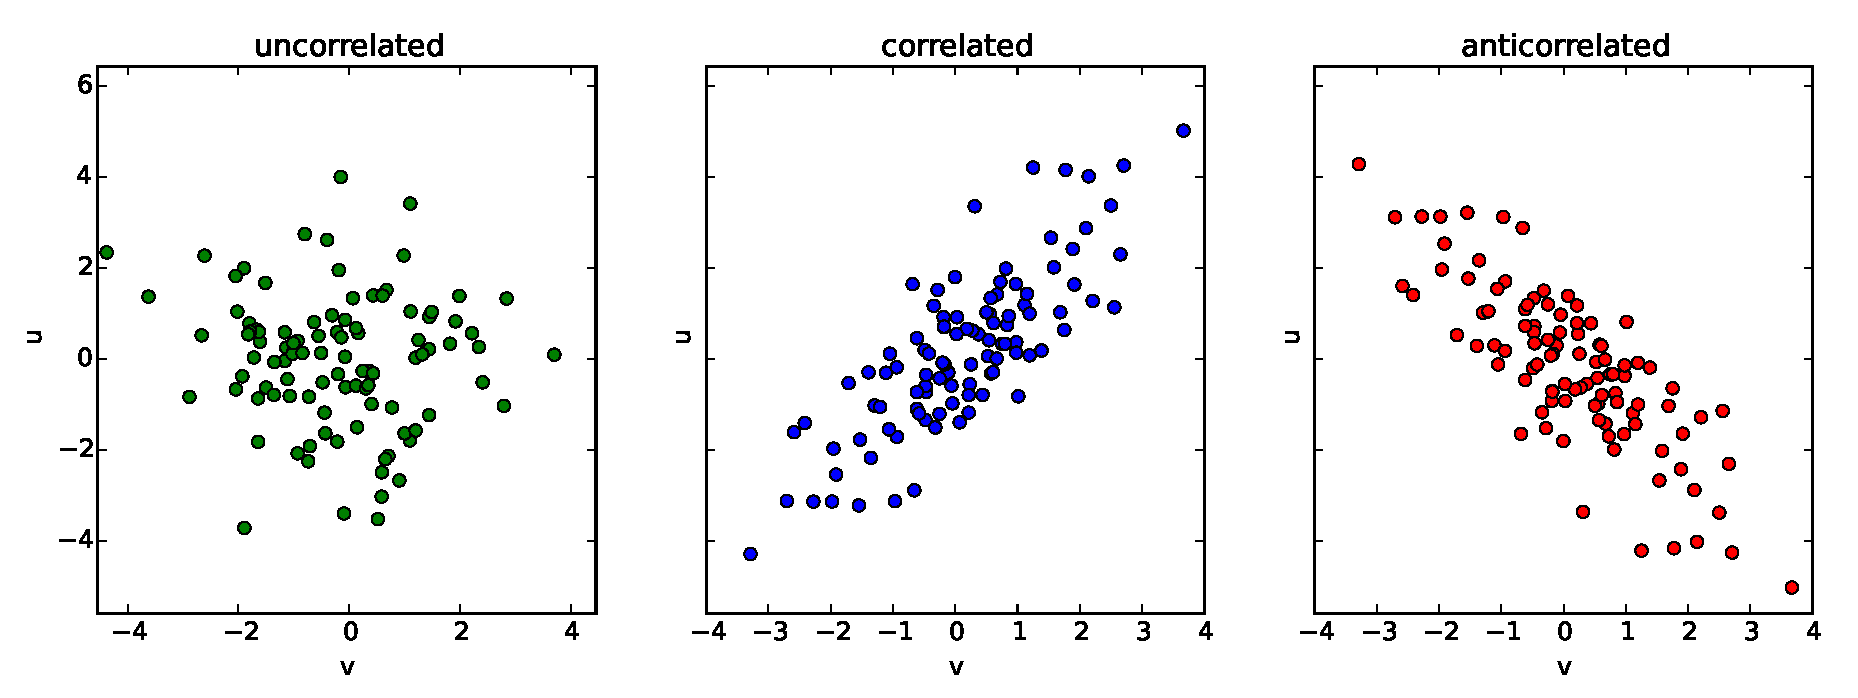
\includegraphics[width=0.95\textwidth]{figures/stats/corr_ex.pdf}
\caption{
Example distributions for
uncorrelated ($\rho \approx 0$),
correlated ($\rho \approx 1$),
and anticorrelated ($\rho \approx -1$)
variables $u$ and $v$ \cite{DougNotes}.
}
\label{fig:stats:corr_ex}
\end{figure}

The covariance matrix,

\begin{align}
  \mathbf{M} = \begin{pmatrix}
    \sigma_1^2   & \cov{1}{2} & \cov{1}{3} & \ldots \\
    \cov{1}{2}   & \sigma_2^2 & \cov{2}{3} & \ldots \\
    \cov{1}{3}   & \cov{2}{3} & \sigma_3^2 & \ldots \\
    \vdots       & \vdots     & \vdots     & \ddots
  \end{pmatrix}\,,
\end{align}

\noindent with elements $M_{ij} = \expval{\left(u_{i} - \bar{u}_{i}\right)\left(u_{j}-\bar{u}_{j}\right)}$
is the higher dimensional extension of the covariance.
We can visualize the covariance between variables with
Gaussian error ellipses given by the probability distribution

\begin{equation}\label{eq:stats:P_error_ellipse_k}
P\left(x_{1},x_{2},\ldots,x_{k}\right) = \frac{1}{(2\pi)^{k/2}}\frac{1}{\abs{\mathbf{M}}^{1/2}}\exp\left[-\frac{1}{2}\left(\mathbf{x}-\bm{\mu}\right)^{\transpose}\mathbf{M}\left(\mathbf{x}-\bm{\mu}\right)\right]\,,
\end{equation}

\noindent where the ellipse semi-axes are directed along the eigenvectors of $\mathbf{M}$.
In two dimensions it is easier to see the equation of the error ellipse itself:

\begin{equation}\label{eq:stats:P_error_ellipse_2}
\begin{split}
P\left(u,v\right) &= \frac{1}{2\pi\sigma_{u}\sigma_{v}}\frac{1}{\sqrt{1-\rho^{2}}}\exp\bigg\{-\frac{1}{2}\bigg[ \\
&\frac{1}{(1-\rho)^{2}}\left(\frac{\left(u-\bar{u}\right)^{2}}{\sigma_{u}^{2}}+\frac{\left(v-\bar{v}\right)^{2}}{\sigma_{v}^{2}}-\frac{2\rho \left(u-\bar{u}\right)\left(v-\bar{v}\right)}{\sigma_{u}\sigma_{v}}\right)\bigg]\bigg\}\,.
\end{split}
\end{equation}
